%=============================--A--=============================%
\subsection{E.3 Análise do sistema QPSK}
\label{sec:analiseQPSK}
\vskip -0.5em
\begin{table}[H]
\caption{Taxa de erro de \textit{bit} em função da \textit{Loop Bandwidth}, para cada \textit{noise voltage}.}
\vskip -0.5em
\label{tab:qpsk}
\hspace*{-0.75cm}\begin{tabular}{|c|c|c|c|c|c|c|c|c|c|}
\hline
Loop BW/Noise & 0.0 & 0.5 & 1.0 & 1.5 & 2.0 & 2.5 & 3.0 & 3.5 & 4.0 \\
\hline\hline
0.006 & \cellcolor{green!25}0.0\% & 1.9\% & 11.1\% & 19.0\% & 28.2\% & 31.5\% & 34.3\% & 36.6\% & 38.0\% \\
\hline
0.012 & \cellcolor{green!25}0.0\% & 1.4\% & 11.1\% & 19.0\% & 27.8\% & 31.0\% & 33.8\% & 35.6\% & 37.5\% \\
\hline
0.018 & \cellcolor{green!25}0.0\% & 1.4\% & 10.6\% & 18.5\% & 26.4\% & 30.6\% & 33.3\% & 36.6\% & \cellcolor{green!25}32.9\% \\
\hline
0.024 & \cellcolor{green!25}0.0\% & 1.4\% & 10.6\% & 18.1\% & 26.9\% & 29.6\% & 33.3\% & \cellcolor{green!25}32.4\% & 35.2\% \\
\hline
0.03 & \cellcolor{green!25}0.0\% & 1.4\% & 9.7\% & 18.1\% & 25.5\% & 29.6\% & \cellcolor{green!25}31.0\% & 35.2\% & 33.8\% \\
\hline
0.036 & \cellcolor{green!25}0.0\% & 0.5\% & 9.3\% & 17.6\% & 25.0\% & 28.2\% & 35.2\% & 35.6\% & 35.2\% \\
\hline
0.042 & \cellcolor{green!25}0.0\% & 0.5\% & 9.3\% & 17.6\% & \cellcolor{green!25}23.1\% & \cellcolor{green!25}27.3\% & 33.8\% & 33.3\% & 41.7\% \\
\hline
0.048 & \cellcolor{green!25}0.0\% & 0.5\% & 9.7\% & 17.6\% & 25.0\% & 30.1\% & 34.7\% & 32.9\% & 46.8\% \\
\hline
0.054 & \cellcolor{green!25}0.0\% & 0.5\% & 9.3\% & 17.1\% & 24.5\% & 29.6\% & 36.6\% & 41.2\% & 37.0\% \\
\hline
0.06 & \cellcolor{green!25}0.0\% & \cellcolor{green!25}0.0\% & 9.7\% & \cellcolor{green!25}15.7\% & 31.0\% & 30.1\% & 38.0\% & 33.8\% & 45.8\% \\
\hline
0.066 & \cellcolor{green!25}0.0\% & \cellcolor{green!25}0.0\% & 7.9\% & 17.1\% & 24.1\% & 36.1\% & 32.9\% & 44.0\% & 37.5\% \\
\hline
0.072 & \cellcolor{green!25}0.0\% & \cellcolor{green!25}0.0\% & 6.9\% & 19.9\% & 26.4\% & 31.5\% & 54.6\% & 44.0\% & 56.0\% \\
\hline
0.078 & \cellcolor{green!25}0.0\% & \cellcolor{green!25}0.0\% & 8.3\% & 17.6\% & 27.8\% & 41.2\% & 34.7\% & 35.2\% & 50.5\% \\
\hline
0.084 & \cellcolor{green!25}0.0\% & \cellcolor{green!25}0.0\% & 8.3\% & 23.1\% & 27.8\% & 45.4\% & 55.1\% & 34.3\% & 52.8\% \\
\hline
0.09 & \cellcolor{green!25}0.0\% & \cellcolor{green!25}0.0\% & 6.9\% & 22.7\% & 25.9\% & 41.7\% & 45.4\% & 48.1\% & 46.8\% \\
\hline
0.096 & \cellcolor{green!25}0.0\% & \cellcolor{green!25}0.0\% & 8.8\% & 25.9\% & 25.9\% & 31.9\% & 36.1\% & 38.4\% & 46.3\% \\
\hline
0.102 & \cellcolor{green!25}0.0\% & \cellcolor{green!25}0.0\% & 6.5\% & 18.5\% & 48.6\% & 30.6\% & 51.4\% & 49.5\% & 48.6\% \\
\hline
0.108 & \cellcolor{green!25}0.0\% & \cellcolor{green!25}0.0\% & \cellcolor{green!25}2.8\% & 17.6\% & 51.4\% & 40.3\% & 52.8\% & 51.9\% & 43.1\% \\
\hline
0.114 & \cellcolor{green!25}0.0\% & \cellcolor{green!25}0.0\% & 3.7\% & 19.9\% & 48.6\% & 37.5\% & 34.3\% & 53.2\% & 38.9\% \\
\hline
0.12 & \cellcolor{green!25}0.0\% & \cellcolor{green!25}0.0\% & 8.8\% & 33.8\% & 27.3\% & 54.6\% & 49.1\% & 50.9\% & 57.4\% \\
\hline
0.126 & \cellcolor{green!25}0.0\% & \cellcolor{green!25}0.0\% & 10.6\% & 20.4\% & 30.6\% & 50.0\% & 54.6\% & 53.7\% & 46.3\% \\
\hline
0.132 & \cellcolor{green!25}0.0\% & \cellcolor{green!25}0.0\% & 8.8\% & 33.3\% & 26.9\% & 34.7\% & 49.5\% & 52.8\% & 50.5\% \\
\hline
0.138 & \cellcolor{green!25}0.0\% & \cellcolor{green!25}0.0\% & 13.9\% & 16.7\% & 27.8\% & 44.9\% & 51.4\% & 47.7\% & 53.2\% \\
\hline
0.144 & \cellcolor{green!25}0.0\% & \cellcolor{green!25}0.0\% & 17.1\% & 16.2\% & 30.6\% & 47.7\% & 47.2\% & 53.2\% & 57.4\% \\
\hline
0.15 & \cellcolor{green!25}0.0\% & \cellcolor{green!25}0.0\% & 15.3\% & 19.0\% & 26.4\% & 50.9\% & 50.5\% & 50.9\% & 51.9\% \\
\hline
0.156 & \cellcolor{green!25}0.0\% & \cellcolor{green!25}0.0\% & 31.0\% & 49.1\% & 33.8\% & 33.3\% & 49.5\% & 54.2\% & 54.2\% \\
\hline
0.162 & \cellcolor{green!25}0.0\% & \cellcolor{green!25}0.0\% & 15.7\% & 50.9\% & 25.9\% & 41.2\% & 47.2\% & 49.1\% & 52.3\% \\
\hline
0.168 & \cellcolor{green!25}0.0\% & \cellcolor{green!25}0.0\% & 16.2\% & 47.7\% & 25.0\% & 36.1\% & 50.9\% & 52.8\% & 53.7\% \\
\hline
0.174 & \cellcolor{green!25}0.0\% & \cellcolor{green!25}0.0\% & 8.3\% & 39.8\% & 33.3\% & 47.2\% & 47.2\% & 55.6\% & 48.6\% \\
\hline
0.18 & \cellcolor{green!25}0.0\% & \cellcolor{green!25}0.0\% & 6.5\% & 35.2\% & 35.2\% & 32.4\% & 53.7\% & 51.4\% & 45.8\% \\
\hline
0.186 & \cellcolor{green!25}0.0\% & \cellcolor{green!25}0.0\% & 10.2\% & 35.6\% & 31.5\% & 53.7\% & 48.6\% & 42.1\% & 50.9\% \\
\hline
0.192 & \cellcolor{green!25}0.0\% & \cellcolor{green!25}0.0\% & 10.2\% & 21.3\% & 32.4\% & 49.1\% & 56.5\% & 52.8\% & 53.7\% \\
\hline
0.198 & \cellcolor{green!25}0.0\% & \cellcolor{green!25}0.0\% & 29.6\% & 19.4\% & 40.3\% & 53.7\% & 52.8\% & 51.9\% & 53.2\% \\
\hline
0.204 & \cellcolor{green!25}0.0\% & \cellcolor{green!25}0.0\% & 29.2\% & 19.4\% & 43.1\% & 52.8\% & 52.3\% & 45.8\% & 47.2\% \\
\hline
0.21 & \cellcolor{green!25}0.0\% & 0.9\% & 10.6\% & 31.0\% & 50.9\% & 53.7\% & 48.6\% & 50.5\% & 42.6\% \\
\hline
0.216 & \cellcolor{green!25}0.0\% & 0.9\% & 30.1\% & 23.6\% & 43.5\% & 47.2\% & 44.9\% & 50.5\% & 40.3\% \\
\hline
0.222 & \cellcolor{green!25}0.0\% & 0.5\% & 10.2\% & 21.8\% & 31.9\% & 29.2\% & 46.3\% & 48.6\% & 51.4\% \\
\hline
0.228 & \cellcolor{green!25}0.0\% & 0.5\% & 7.4\% & 22.2\% & 36.6\% & 48.1\% & 48.6\% & 49.1\% & 53.7\% \\
\hline
0.234 & \cellcolor{green!25}0.0\% & 0.5\% & 7.9\% & 21.8\% & 32.4\% & 51.4\% & 51.9\% & 50.0\% & 51.4\% \\
\hline
0.24 & \cellcolor{green!25}0.0\% & 0.5\% & 6.0\% & 47.2\% & 38.0\% & 47.7\% & 48.1\% & 44.9\% & 44.9\% \\
\hline
0.246 & \cellcolor{green!25}0.0\% & \cellcolor{green!25}0.0\% & 6.5\% & 48.1\% & 51.9\% & 45.4\% & 47.7\% & 44.0\% & 51.9\% \\
\hline
0.252 & \cellcolor{green!25}0.0\% & 0.5\% & 11.1\% & 50.0\% & 46.3\% & 55.1\% & 54.2\% & 52.3\% & 42.6\% \\
\hline
\end{tabular}
\end{table}

%---
\begin{figure}[H]
    \centering
    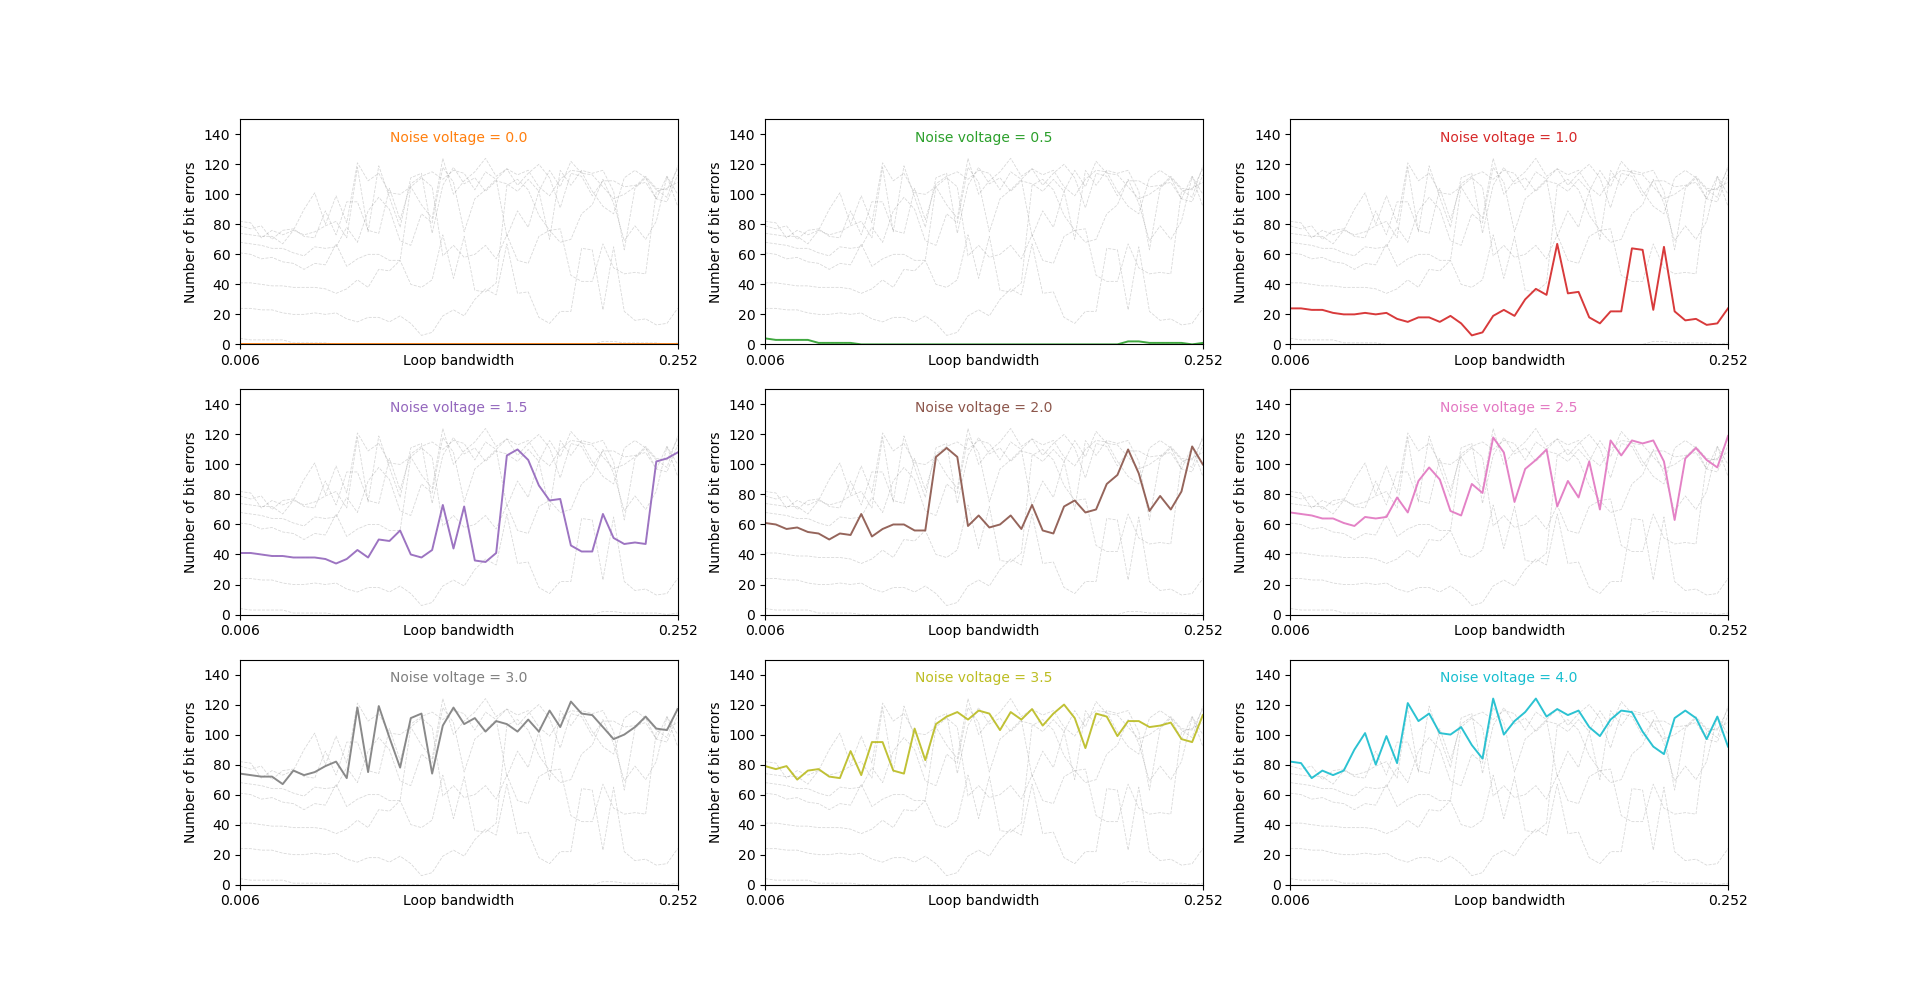
\includegraphics[width=1\linewidth]{img/analise/QPSK_9.png}
    \caption{Evolução do número de erros de bit para cada \textit{noise voltage}, em função da \textit{Loop Bandwidth}.}
    \label{fig:qpsk9}
\end{figure}

\noindent\fcolorbox{black}{white}{%
        \minipage[t]{\dimexpr\linewidth-2\fboxsep-2\fboxrule\relax}
            \textbf{Nota} $\rightarrow$ Os resultados e observações são bastante análogos à versão BPSK, pelo que se seguem as mesmas ilações. Salienta-se somente, para reforçar a ideia, que em média, a taxa de erro de \textit{bit} para cada patamar de ruído impõe precisamente a mesma evolução que no caso exposto anteriormente (vide \hyperref[fig:bpsk9]{Fig. E1} e \hyperref[tab:bpsk]{Tab. E1}). 
        \endminipage}